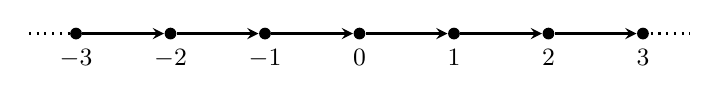
\begin{tikzpicture}[scale=1.2]
\foreach \x in {-3,...,3} {
    \node[circle, fill=black, inner sep=1.5pt, label=below:{\small \(\x\)}] (n\x) at (\x, 0) {};
}
\foreach \x in {-3,...,2} {
    \pgfmathtruncatemacro{\y}{\x+1}
    \draw[->, >=stealth, thick] (n\x) -- (n\y);
}
\draw[dotted, thick] (-3.5, 0) -- (-3, 0);
\draw[dotted, thick] (3, 0) -- (3.5, 0);
\end{tikzpicture}
